%!TEX program = xelatex
\documentclass[12pt, a4paper]{article}

\usepackage[dvipsnames]{xcolor}

\usepackage{fancyhdr}
\usepackage{extramarks}
\usepackage{amsmath}
\usepackage{amsthm}
\usepackage{amsfonts}
\usepackage{tikz}
\usepackage[plain]{algorithm}
\usepackage{algpseudocode}

\usepackage{ctex}
\usepackage{indentfirst}
\usepackage{wrapfig}
\usepackage{upgreek}
\usepackage{subfigure}
\ctexset {today=old}
\usetikzlibrary{automata,positioning,shapes.geometric,arrows.meta,patterns,calc}
\numberwithin{equation}{section}

%
% Basic Document Settings
%

\topmargin=-0.25in
\evensidemargin=0in
\oddsidemargin=0in
\textwidth=6.5in
\textheight=9.2in
\headsep=0.25in

\linespread{1.1}

\pagestyle{fancy}
\lhead{\hmwkAuthorName}
\chead{\hmwkClass : \hmwkTitle}
\rhead{\firstxmark}
\lfoot{\lastxmark}
\cfoot{\thepage}

\renewcommand\headrulewidth{0.4pt}
\renewcommand\footrulewidth{0.4pt}

\setlength{\parindent}{2em}  % 2em代表首行缩进两个字符

%
% Create Problem Sections
%

\newcommand{\enterProblemHeader}[1]{
    \nobreak\extramarks{}{Problem \arabic{#1} continued on next page\ldots}\nobreak{}
    \nobreak\extramarks{Problem \arabic{#1} (continued)}{Problem \arabic{#1} continued on next page\ldots}\nobreak{}
}

\newcommand{\exitProblemHeader}[1]{
    \nobreak\extramarks{Problem \arabic{#1} (continued)}{Problem \arabic{#1} continued on next page\ldots}\nobreak{}
    \stepcounter{#1}
    \nobreak\extramarks{Problem \arabic{#1}}{}\nobreak{}
}

% \setcounter{secnumdepth}{0}
\newcounter{partCounter}
\newcounter{homeworkProblemCounter}
\setcounter{homeworkProblemCounter}{0}
% \nobreak\extramarks{Problem \arabic{homeworkProblemCounter}}{}\nobreak{}

%
% Homework Problem Environment
%
% This environment takes an optional argument. When given, it will adjust the
% problem counter. This is useful for when the problems given for your
% assignment aren't sequential. See the last 3 problems of this template for an
% example.
%
\newenvironment{homeworkProblem}[1][-1]{
    \ifnum#1>0
        \setcounter{homeworkProblemCounter}{#1}
    \fi
    \section{Problem \arabic{homeworkProblemCounter}}
    \setcounter{partCounter}{1}
    \enterProblemHeader{homeworkProblemCounter}
}{
    \exitProblemHeader{homeworkProblemCounter}
}

%
% Homework Details
%   - Title
%   - Due date
%   - Class
%   - Section/Time
%   - Instructor
%   - Author
%

\newcommand{\hmwkTitle}{Mechanical Wave}
\newcommand{\hmwkDueDate}{\today}
\newcommand{\hmwkClass}{University Physics}
\newcommand{\hmwkClassTime}{}
\newcommand{\myUniversiy}{Wuhan University}
\newcommand{\hmwkAuthorName}{\textbf{Lai Wei}}

%
% Title Page
%

\title{
    \vspace{2in}
    \textmd{\textbf{\hmwkClass:\ \hmwkTitle}}\\
    \normalsize\vspace{0.1in}\small{Date: \hmwkDueDate}\\
    \vspace{0.1in}\large{\textit{\myUniversiy}}
    \vspace{3in}
}

\author{\hmwkAuthorName}
\date{}

\renewcommand{\part}[1]{\textbf{\large Part \Alph{partCounter}}\stepcounter{partCounter}\\}

%
% Various Helper Commands
%

% Useful for algorithms
\newcommand{\alg}[1]{\textsc{\bfseries \footnotesize #1}}

% % For derivatives
% \newcommand{\deriv}[1]{\frac{\mathrm{d}}{\mathrm{d}x} (#1)}

% For partial derivatives
\newcommand{\pderiv}[2]{\frac{\partial}{\partial #1} (#2)}

% Integral dx
\newcommand{\dx}{\mathrm{d}x}

% Alias for the Solution section header
\newcommand{\solution}{\textbf{\large Solution}}

% Probability commands: Expectation, Variance, Covariance, Bias
\newcommand{\E}{\mathrm{E}}
\newcommand{\Var}{\mathrm{Var}}
\newcommand{\Cov}{\mathrm{Cov}}
\newcommand{\Bias}{\mathrm{Bias}}

% 我的newcommand
\newcommand{\degree}{^{\circ}}
\newcommand{\arrow}{-{Stealth[length=4mm,width=2mm]}}
\newcommand{\rmd}{\mathrm{~d}}
\newcommand{\deriv}[2]{\frac{\rmd #1}{\rmd #2}}
\renewcommand{\parallel}{\mathrel{/\mskip-2.5mu/}}

\begin{document}

\maketitle

\pagebreak

% 设置页码格式是罗马数字
\pagenumbering{roman}

% 生成目录
\tableofcontents

% \newpage 
% \mbox{}
% \newpage

\pagebreak

% 设置页码格式是阿拉伯数字
\pagenumbering{arabic}

\pagebreak

    振动与波动的关系:
    振动是激发波动的波源;波动是振动的传播过程。

\section{机械波的产生和传播}

\subsection{机械波的基本概念}

\subsubsection{产生条件}

    \textbf{波}是振动状态再空间的传播过程。

    \textbf{机械波}是机械振动在弹性介质中的传播过程。

    \textbf{电磁波}是交变电场在空间的传播过程。

    \textbf{弹性介质}(elastic medium):由无穷多个质元通过弹性力结合再一起形成的连续介质。

    要产生机械波,必须满足两个条件:

    \begin{enumerate}
        \item 要有波源(即振动源);
        \item 要有能够传播机械振动的弹性介质。
    \end{enumerate}

    机械波与电磁波的共同特征:

    \begin{enumerate}
        \item 具有一定的传播速度;
        \item 能够产生干涉、衍射现象;
        \item 伴随着能量的传播;
        \item 具有相似的数学表达式。
    \end{enumerate}

\subsubsection{横波和纵波}

    \textbf{横波}:质点的振动方向与波的传播方向垂直。
    横波中凸起的位置称为波峰,下凹的位置称为波谷。

    \textbf{纵波}(又称为疏密波):质点的振动方向与波的传播方向平行。

    在机械波中,横波只能在固体中出现;纵波可在气体、液体和固体中出现。
    空气中的声波是纵波。液体表面的波动情况较复杂,不是单纯的纵波或横波。

\subsubsection{波的几何描述}

    波阵面(波面, wave surface):相位相同的点连成的面;

    波线(波射线, wave ray):波的传播方向。

    \[
        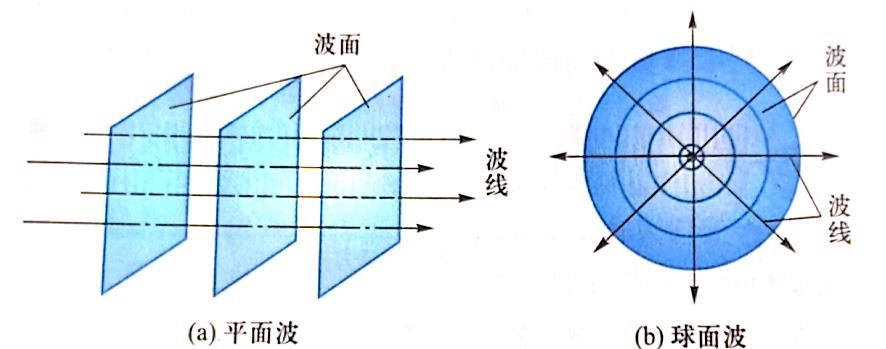
\includegraphics[scale=0.4]{Chapter 07 images/pic1.jpg}
    \]

\subsection{描述机械波的物理量}

\subsubsection{波速}

    单位时间内振动状态在介质中传播的距离称为波的传播速度,简称波速。
    在弹性介质中,机械波的传播速度取决于介质的惯性和弹性,
    也就是取决于介质的密度和弹性模量,与波源在介质中的运动速度无关。

    在拉紧的弹性绳索中,横波的传播速度为

    \begin{align}
        u = \sqrt{\frac{F }{\lambda}}
    \end{align}

    式中\(F \)为绳中的张力,\(\lambda\)是绳的质量线密度。

    在固体中,既可以传播横波,也可以传播纵波,它们的传播速度分别为

    \begin{equation}
        u=\sqrt{\frac{G}{\rho}} \quad \text{(横波)}
    \end{equation}

    \begin{equation}
        u=\sqrt{\frac{E}{\rho}} \quad(\text{(纵波)})
    \end{equation}
    
    式中\(\rho\)是固体的密度,\(G\)和\(E\)分别是固体的切变模量(shear modulus)和杨氏模量\\
    (Young's modulus),它们是反应材料形变和內应力关系的物理量,其单位都是\(\mathrm{N \cdot m^{-2}}\)。

    在液体和液体中,纵波的传播速度为

    \begin{equation}
        u=\sqrt{\frac{K}{\rho}}
    \end{equation}

    式中\(K\)为介质的体积模量,\(\rho\)是气体或液体的密度。

    对于理想气体,根据分子动理论和热力学理论,可以证明理想气体中声波的传播速度为

    \begin{equation}
        u=\sqrt{\frac{\gamma p}{\rho}}=\sqrt{\frac{\gamma R T}{M}}
        \label{7-1-5}
    \end{equation}

    式中\(M\)是气体分子的摩尔质量,是气体的摩尔定压热容与摩尔定容热容之比,
    简称摩尔热容比,\(p\)是气体的压强,\(T\)是热力学温度,\(R \)是摩尔气体常量。
    式\ref{7-1-5}表明,气体中声波的传播速度不仅与气体的性质有关,还与温度有关。

\subsubsection{波长、周期和频率}

    \textbf{波长}(wave length):波的传播方向上相邻两振动状态完全相同的质点间的距离(一完整波的长度),
    用\(\lambda\)表示。

    \textbf{周期}:波传播一个波长的距离所用的时间,用\(T \)表示。

    波速\(u \)、波长\(\lambda\)和周期\(T \)三者之间有如下关系:

    \begin{equation}
        u=\frac{\lambda}{T}
        \label{7-1-6}
    \end{equation}

    \textbf{频率}:单位时间内波向前传播的完整波的数目,是周期的倒数,用\(\nu\)表示。
    于是式\ref{7-1-6}\\可改写为

    \begin{equation}
        u=\nu \lambda
    \end{equation}

    当波源和弹性介质没有相对运动(仅仅在介质中做振动)时,波源每做一次完全振动,
    波就会向前传播一个波长的距离,这表明波源的振动周期和振动频率在数值上与波的周期和波的频率是相等的,
    即两组物理量可以通用。如果波源与介质有相对运动,则两组物理量有差异,不可通用。

\end{document}
